\PassOptionsToPackage{unicode=true}{hyperref} % options for packages loaded elsewhere
\PassOptionsToPackage{hyphens}{url}
%
\documentclass[10pt,]{article}
\usepackage{lmodern}
\usepackage{subfigure}
\usepackage{amssymb,amsmath}
\usepackage{ifxetex,ifluatex}
\usepackage{fixltx2e} % provides \textsubscript
\ifnum 0\ifxetex 1\fi\ifluatex 1\fi=0 % if pdftex
  \usepackage[T1]{fontenc}
  \usepackage[utf8]{inputenc}
  \usepackage{textcomp} % provides euro and other symbols
\else % if luatex or xelatex
  \usepackage{unicode-math}
  \defaultfontfeatures{Ligatures=TeX,Scale=MatchLowercase}
\fi
% use upquote if available, for straight quotes in verbatim environments
\IfFileExists{upquote.sty}{\usepackage{upquote}}{}
% use microtype if available
\IfFileExists{microtype.sty}{%
\usepackage[]{microtype}
\UseMicrotypeSet[protrusion]{basicmath} % disable protrusion for tt fonts
}{}
\IfFileExists{parskip.sty}{%
\usepackage{parskip}
}{% else
\setlength{\parindent}{0pt}
\setlength{\parskip}{6pt plus 2pt minus 1pt}
}
\usepackage{hyperref}
\hypersetup{
            pdftitle={Tri crêpe},
            pdfborder={0 0 0},
            breaklinks=true}
\urlstyle{same}  % don't use monospace font for urls
\usepackage[margin=3cm]{geometry}
\usepackage{graphicx,grffile}
\makeatletter
\def\maxwidth{\ifdim\Gin@nat@width>\linewidth\linewidth\else\Gin@nat@width\fi}
\def\maxheight{\ifdim\Gin@nat@height>\textheight\textheight\else\Gin@nat@height\fi}
\makeatother
% Scale images if necessary, so that they will not overflow the page
% margins by default, and it is still possible to overwrite the defaults
% using explicit options in \includegraphics[width, height, ...]{}
\setkeys{Gin}{width=\maxwidth,height=\maxheight,keepaspectratio}
\setlength{\emergencystretch}{3em}  % prevent overfull lines
\providecommand{\tightlist}{%
  \setlength{\itemsep}{0pt}\setlength{\parskip}{0pt}}
\setcounter{secnumdepth}{0}
% Redefines (sub)paragraphs to behave more like sections
\ifx\paragraph\undefined\else
\let\oldparagraph\paragraph
\renewcommand{\paragraph}[1]{\oldparagraph{#1}\mbox{}}
\fi
\ifx\subparagraph\undefined\else
\let\oldsubparagraph\subparagraph
\renewcommand{\subparagraph}[1]{\oldsubparagraph{#1}\mbox{}}
\fi

% set default figure placement to htbp
\makeatletter
\def\fps@figure{htbp}
\makeatother
\geometry{
 a4paper,
 total={170mm,257mm},
 left=20mm,
 top=20mm,
}

\title{Tri crêpe}
\date{}

\begin{document}
\maketitle

\hypertarget{principe}{%
\section{Principe}\label{principe}}

On dispose d'un empilement de crêpes que l'on souhaite les ranger dans
l'ordre croissant, la crêpe la plus petite en haut.

\begin{figure}
	\centering
	\subfigure[État initial]{\label{sub1}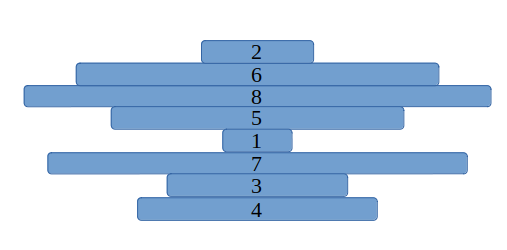
\includegraphics[width=160]{schema1.png}}
	\subfigure[État final]{\label{sub2}	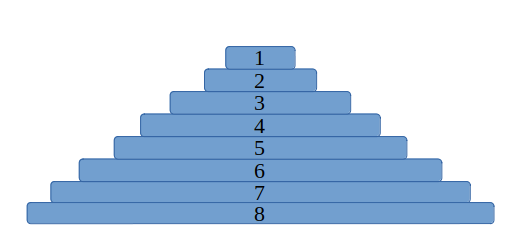
\includegraphics[width=160]{schema2.png}}
	\caption{État initial et état final}
\end{figure}

Pour cela, vous ne disposez que d'un seul type opération : glisser une
spatule sous une crêpe et retourner tout l'empilement de crêpes se
trouvant sur votre spatule.

\begin{figure}
    \centering
    \subfigure{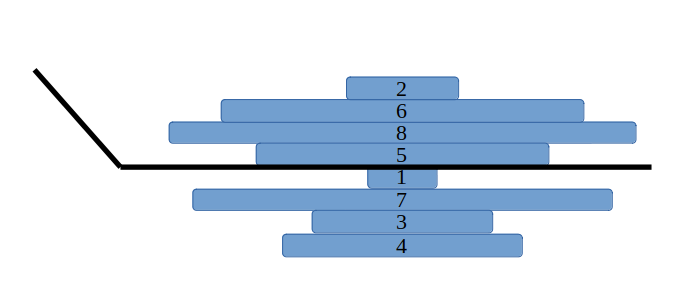
\includegraphics[width=160]{schema3.png}}
    \subfigure{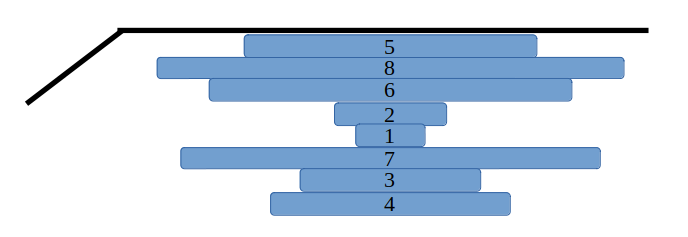
\includegraphics[width=160]{schema4.png}}
    \caption{Opération disponible}
\end{figure}

La \emph{figure 2} montre l'opération que l'on
dispose.

\hypertarget{objectif}{%
\subsubsection{Objectif}\label{objectif}}

L'objectif est de rédiger un algorithme permettant de trier un
empilement de crêpes.

\hypertarget{consigne}{%
\subsection{Consigne}\label{consigne}}

A l'aide du matériel mis à disposition, rédiger (sur feuille) un
algorithme en français, résultant de vos manipulations.

\hypertarget{matuxe9riel-mis-uxe0-disposition}{%
\subsubsection{Matériel mis à
disposition}\label{matuxe9riel-mis-uxe0-disposition}}

\begin{itemize}
\tightlist
\item
  Lot de crêpes de différentes tailles
\end{itemize}

\hypertarget{a-rendre}{%
\subsubsection{A rendre}\label{a-rendre}}

Vous devez rendre un compte rendu de vos manipulations. Il est attendu
la rédaction d'un algorithme, ce dernier sera rédigé en français.

\end{document}
